\section{Playaround}
% This is unique for class presentation.
\begin{frame}{\LaTeX Meeting-protocol}{Can be found \where}
    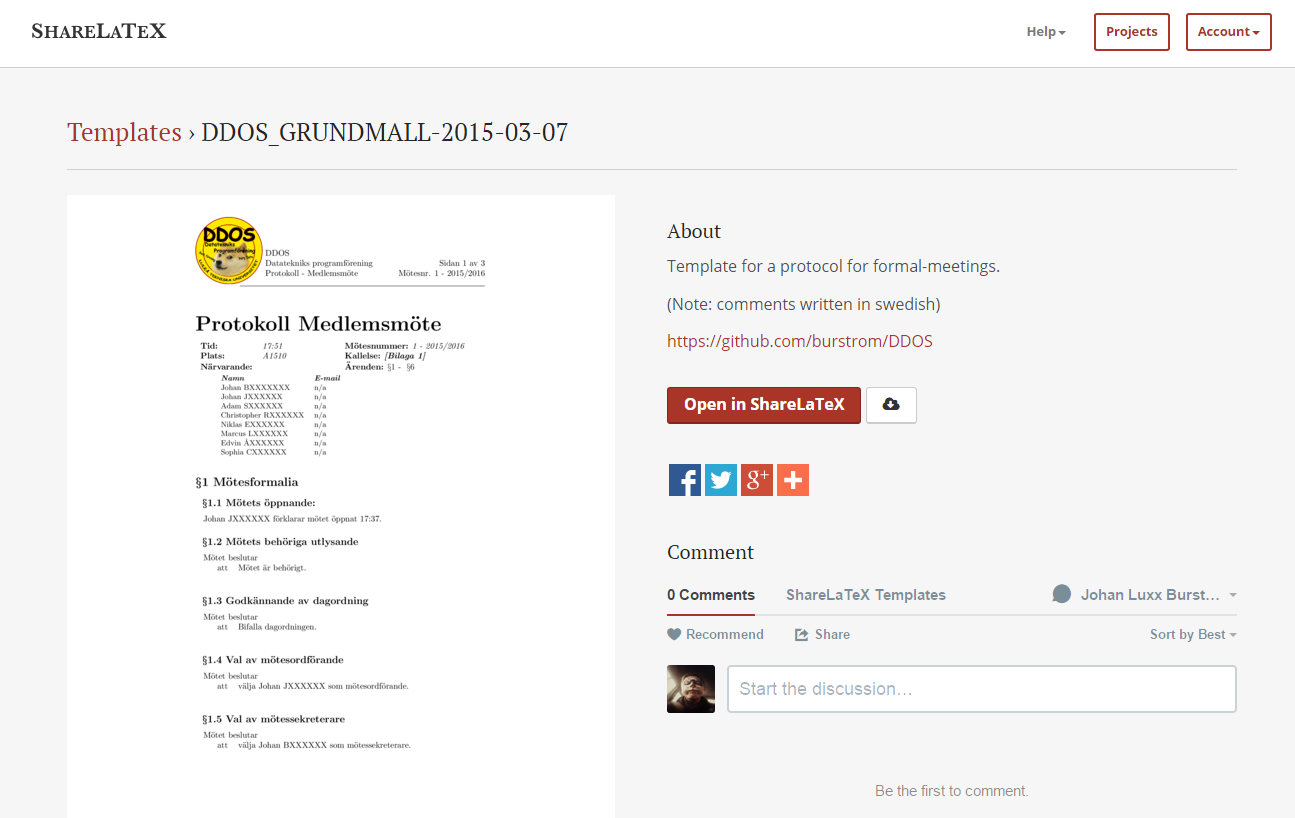
\includegraphics[width=\textwidth]{img/3-protlatex.png}
\end{frame}

\begin{frame}{\LaTeX Meeting-protocol}{Can be found \where}
    Take some time and download the template also. \\ \ \\ \ \\
    \small This link also works: \\ \ \\ \ \\
    \normalsize
    \texttt{http://tinyurl.com/ddoslatex}
\end{frame}

\begin{frame}{\LaTeX Meeting-protocol}
	Things to notice: \\ \ 
	\begin{itemize}
	\item \textbackslash newcommand
	\item \textbackslash minipage
	\end{itemize} 
\end{frame}

\subsection{Packages}
\begin{frame}[fragile]{Good packages to lookup.}
	\begin{block}{The following packages are great!}
	\begin{lstlisting}
		fancyhdr,
		pdfpages,
		calc
	\end{lstlisting}
	\end{block}
	\begin{block}{Fancyhdr}
	Gives header, margin notes, and much more.
	\textcolor{blue}{http://texdoc.net/texmf-dist/doc/latex/fancyhdr/fancyhdr.pdf}
	\end{block}
	\begin{block}{pdfpages}
	lets you include pdf-files, very useful for attachments!
	\textcolor{blue}{http://texdoc.net/texmf-dist/doc/latex/pdfpages/pdfpages.pdf}
	\end{block}	

\end{frame}
\begin{frame}[fragile]{Packages continued..}
	\begin{block}{calc}
	Adds expressions to perform arithmetic on arguments.
		Also important to use if you want to use counters!
	\textcolor{blue}{http://texdoc.net/texmf-dist/doc/latex/pdfpages/pdfpages.pdf}
	\end{block}
\end{frame}

\subsection{Counters}
\begin{frame}[fragile]{Counters can be useful for manually fixing values.}
	\begin{block}{To create a counter}
	   	\begin{lstlisting}
		\newcounter{cnter} % First initiate the counter
		\setcounter{cnter}{0} % default 0, if it's not set manually
		\end{lstlisting}
   \end{block}
   	\begin{block}{To use our counter}
	   	\begin{lstlisting}
			\thecnter % Returns the value of the counter
			\stepcounter{cnter} % increases the value
		\end{lstlisting}
   \end{block}
\end{frame}